%we have some fixed parameters such as light control on or off. Mimics intersection lights.\\
%Whether simulated vehicles are able to turn or not.\\
%We have different max speeds - 60 or 40 km per hour approach. This translates to lower speeds %during turns (roughly half).\\

%tests are different combinations of above parameters. And results are measured in collisions, cars spawned, cars reaching destination, and time before deadlock.\\
%Deadlock is the situation where cars have been stuck for a period of time in the `intersection zone' without entering or leaving.

%To test the implementation of our system we ran some simulations 
To compare performances of the system over different paradigms and with different factors, we ran
multiple experimental simulations.
The factors that we changed over the different tests are from three classes: the regulation, the speed of the cars, and the complexity.

For regulation it is meant the use of  a traffic light regulated intersection versus an unregulated intersection pure reactive approach.
It is worth pointing out that when using traffic lights, the agents of the system still make use of their underlying reactive layer for obstacle avoidance.
They also do so in the same way as they do without the traffic lights enabled.
Traffic lights have the only purpose of regulating traffic flow by limiting its direction and changing it at fixed intervals.

Regarding complexity, it can be increased by allowing the cars to turn in order to reach any destination, or we can use a simpler system where cars only wish to reach the opposite destination, going straight.

The car speed is changed between three base cases: slow ( 30 km/h), medium (40 km/h) and fast (60 km/h).
For comparison, it is worth mentioning that the advised speed when making a 90 degree turn inside urban areas is around or below 30 km/h. \textbf{a reference would be nice} %todo find reference

When simulating with traffic lights enabled, we test two intervals of time that regulate the duration of the green light.
We have an interval window of approximately 1 minute, that reflects a realistic scenario according to our observation of real life intersections.
We also test a much shorter window of 20 seconds, that should improve performance under the assumptions that:
\begin{enumerate}
\item autonomous vehicles can react faster than human drivers, so they can start moving immediately after the traffic light turns green compared to human drivers which could be slow or distracted;
\item shorter windows of time allow the traffic to be managed evenly, since traffic is evenly generated from the different directions.
\end{enumerate}

\subsection{Experimental results}

We measure performance of the systems mainly in terms of throughput, namely the amount of cars that get through the intersection per minute.\\
However, we also account for other factors, like the amount of collisions, the amount of deadlock situations, the time at which these occur and the frequency of these events.\\
\noindent
A deadlock is the condition in which cars have been stuck in the intersection zone with no one entering or leaving for a period of time (about 10 seconds). This is represented in figure \ref{fig:deadlock}.\\

\begin{figure}
\centering
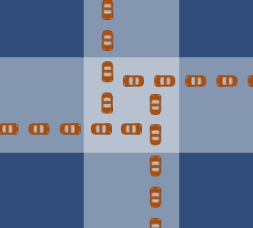
\includegraphics[height=120px]{img/deadlock2}
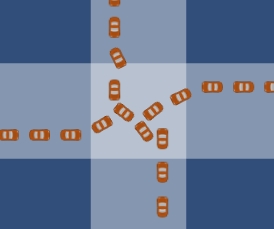
\includegraphics[height=120px]{img/deadlock}
\caption{Two deadlocks: no car is able to advance and the intersection is blocked}
\label{fig:deadlock}
\end{figure}
\noindent
To test the implementation of our system we also account for information such as the number of cars spawned, number of cars "lost" (not reaching the correct destination) and the number of cars present in the intersection zone at the occurrence of a deadlock or collision.


On the other hand, we don't take into account neither fuel consumption nor gas emissions in this simulation, which would be relevant parameters for real life applications.

\subsubsection{Throughput}

\begin{figure}
\centering
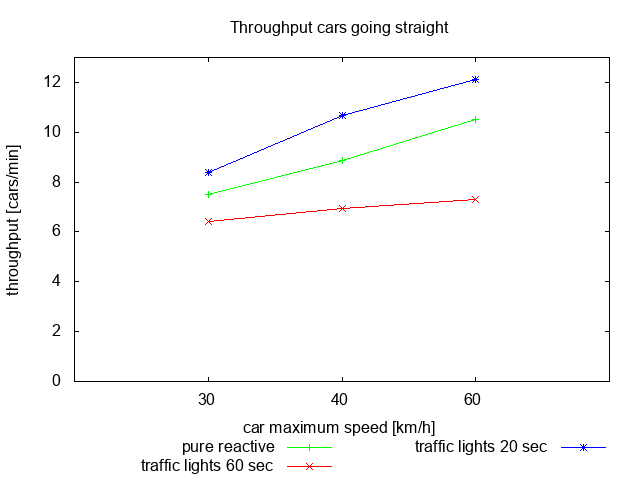
\includegraphics[scale=0.35]{img/plot_throughstraight}
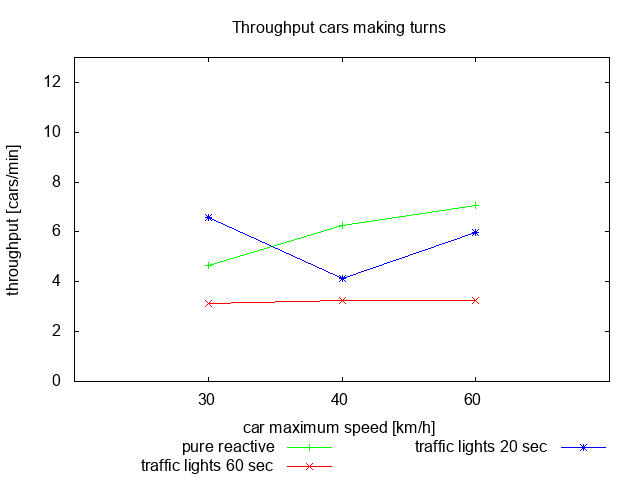
\includegraphics[scale=0.35]{img/plot_throughturns}
\caption{Throughputs in comparison: cars only move forward (left) versus cars able to turn (right). Pure reactive approach in green, traditional traffic light approach in red and fast traffic light approach in blue}
\label{fig:throughput}
\end{figure}

The graphs in figure \ref{fig:throughput} show the different throughputs of the system running with different factors.
%The graphs are divided by paradigm: the first one shows a pure reactive approach, while the second and the third one show the system working with traffic lights in intervals of 60 and 20 seconds respectively.
The graphs are divided by complexity: the first one shows the different throughputs when the cars can only go straight, while in the second one the cars can also make turns.\\

%For each graph, two versions of the same paradigm are compared: one where the agents only go straight and another one where they can turn in any directions.

For each graph, three regulation approaches are compared: the pure reactive approach, and the two with traffic lights, with light intervals of 60 and 20 seconds respectively.\\
Finally, for each case multiple tests are ran with cars moving at different speeds, that are represented on the x axis.\\

The first thing that can be evinced from the graphs is that when adding complexity, namely the ability to turn, throughput drops in all three cases.\\
%This can be easily seen in the fact that in every graph the darkest line (cars going straight) is above the lightest one.
This is mostly due to the fact that deadlocks are produced at a higher rate when turning is enabled, as will be later discussed.

The main purpose of the graph though, is the comparison between the pure reactive approach (green), the traffic light approach (red), and the approach with traffic lights with a faster switch interval (blue).

In the first graph (on the \textbf{left}, figure \ref{fig:throughput}) the pure reactive approach achieves better throughput than the traditional traffic light approach, but they are both surpassed by the faster traffic light system.

When the cars can turn (\textbf{right} figure), throughput is lowered by approximately half, and the pure reactive seems to be the best system, followed by the fast traffic-light system and the traditional one in last position.

\subsubsection{Deadlocks}

\begin{figure}
\centering
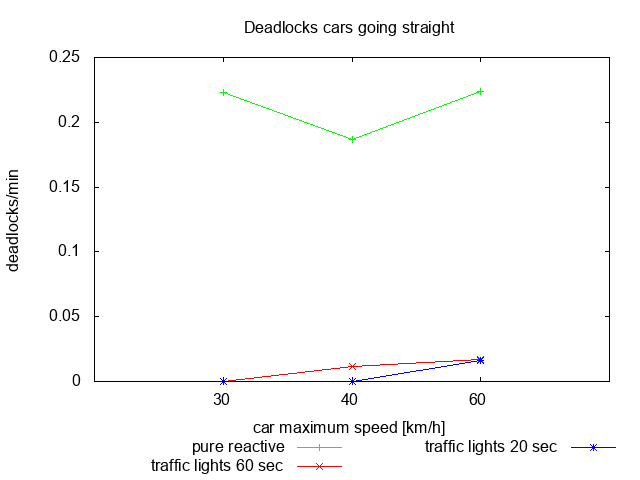
\includegraphics[scale=0.35]{img/plot_deadlocksstraight}
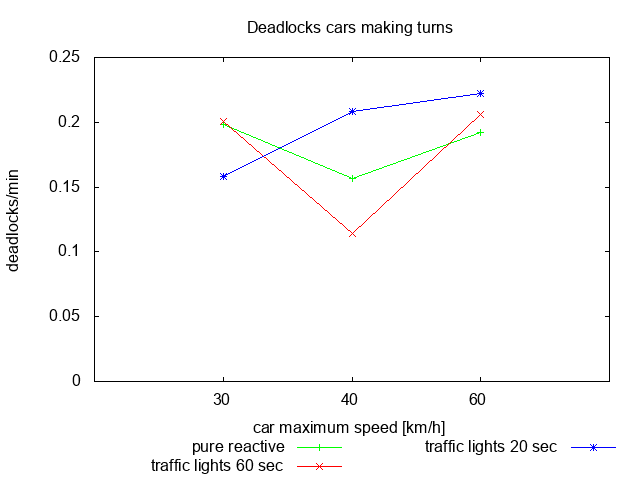
\includegraphics[scale=0.35]{img/plot_deadlocksturns}
\caption{Deadlocks' frequencies in comparison}
\label{fig:deadlocks}
\end{figure}

\begin{figure}
\centering
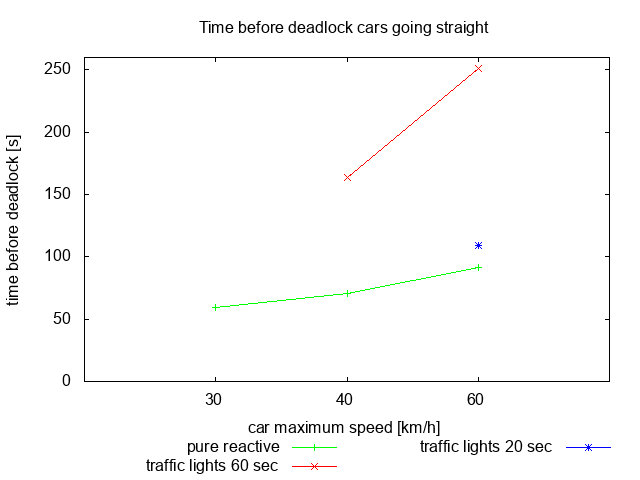
\includegraphics[scale=0.35]{img/plot_dtimestraight}
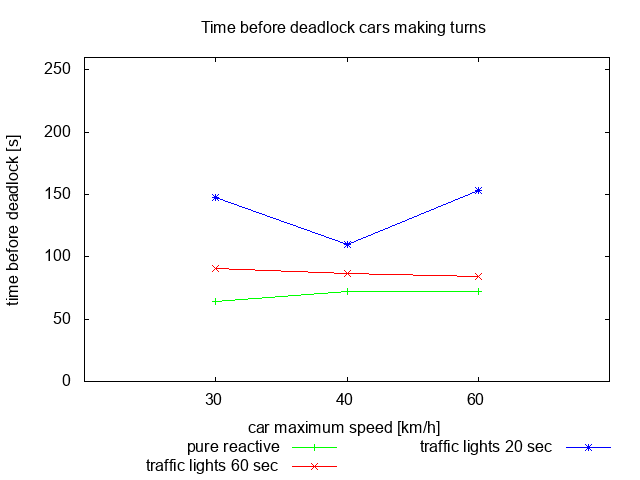
\includegraphics[scale=0.35]{img/plot_dtimeturns}
\caption{Time before deadlock in comparison}
\label{fig:dtime}
\end{figure}

Figure \ref{fig:deadlocks} shows the occurrence of deadlocks per minute in the various simulations.\\
Figure \ref{fig:dtime} shows the average time before a deadlock occurs.
\newline

The throughput results alone are not precise indicators of performance of the systems.
These results only indicate the performance of the system when actively sorting traffic, which doesn't happen when deadlocks occur.

%During the simulations deadlock situations were often present.
After a deadlock, the simulation is no longer able to produce throughput, as the entire intersection is blocked.
Instead of using standard time windows for the experiments and comparing throughput during those, the simulations were stopped after the occurrence of deadlocks.

This approach achieves a better throughput information for the system, but it only represents the throughput when the system works.
This is why it is not sufficient to represent the performance of the system, hence we also need to look at deadlock information.


It is clear from these graphs (figure \ref{fig:deadlocks}) that when the cars can only go \textbf{forward}, deadlocks are much more frequent in the pure reactive system.
Not only they happen more, but they are likely to occur in less time.


When cars can \textbf{turn}, deadlocks are frequent for every study case, at a comparable level.
The only case when values differ significantly is when cars move at an average speed, while when they move slow or fast they present similar behaviours.
In regards to the times, deadlocks are likely to happen in less time for the pure reactive approach, while the system that can last the longest is the fast traffic-light one.


\subsubsection{Performance discussion}
From these results, it is clear that none of the tested approaches is perfect yet.
Overall, the system using traffic lights at a low switch rate seems to perform better than the other ones.
This is especially true when cars can only go straight, when the throughput is maximised and little to no deadlocks occur.

As for the unregulated version, it performs well when cars go straight, but about 1 out of 4 times a deadlock occurs in the first minute of functioning.

When cars can turn, performance drops both in terms of throughput and deadlock avoidance.

This is due to the fact that the reactive approach that we are testing, being it regulated by traffic lights or not, is not "intelligent" and can not manage itself with consciousness.
It is in fact very close to a greedy approach, in which agents (cars) move forward through their path as soon as they have space to do so.
This is very likely to result in cars getting in the way of other cars without being able to continue, thus blocking the intersection.


It all comes down to shared resource management in a concurrent environment.
The intersection is the shared resource at any given time, and the cars need to handle the access to it in a way that it is assured that they can leave.
The more cars are simultaneously in the intersection at a given time, the more likely it is to form a deadlock.
If the cars can turn in any direction it is even more likely due to the fact that a car making a turn will pass through a position where it can block at least two lanes at a time.
\newline

Another interesting aspect to discuss is that the deadlock frequency seems to follow a v-shaped pattern.
This basically means that the frequency is higher at low and high speeds then it is at medium speed.

We can interpret this as the fact that slow cars are slower to move out of the way and can deadlock faster.
Fast cars are faster to move out of the way, but also to reach for a position where they can potentially block others when the center is crowded.
\newline

Finally, one may wonder how deadlocks can happen in traffic-light regulated intersections if cars can only go straight.
Regardless of how infrequently this happens, the value is not zero.
This can happen in two different ways.

First of all, when running at high speeds some cars just can't stop in time at a red traffic light, and will keep going after they surpass it.
This will have cars traverse the intersection perpendicularly to the direction where the rest of the traffic is flowing, potentially blocking the way.

Another reason is that cars can clear the intersection slowly when lights change.
Traffic lights are switched with an offset of 3 seconds, during which all lights turn red to make sure the intersection is clear once they change back. 
This offset sometimes is not enough, especially when cars move slowly or the intersection is very crowded.\\
Also in this case cars will traverse perpendicularly.

An example of this behaviour is shown in figure \ref{fig:dead-start}.

\begin{figure}
\centering
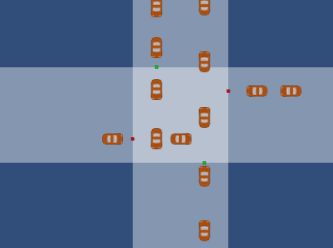
\includegraphics[scale=0.65]{img/deadlock-start-str}
\caption{Car traversing the intersection perpendicularly} 
\label{fig:dead-start}
\end{figure}


\subsubsection{Collisions}
Another parameter that we wanted to measure is the likelihood of collisions to occur.
While an intersection management system should have zero tolerance for deadlocks and collisions, this was not achieved during our simulations.

Figure \ref{fig:collisions} shows the number of collisions happening per minute for the different systems.
These graphs have the same scale as the ones representing the frequency of deadlocks.
At a quick glance, it is immediately visible that collisions are much less frequent than deadlocks.
Also, when cars can turn there is a visible correlation with speed and number of collisions, especially in regulated systems.
We already discussed that cars moving very fast don't have enough break distance to stop before a red light, and keeps going.
This behaviour can cause collisions as well as deadlocks when the collision avoidance fails due to particular timings or velocities before impact.


\begin{figure}
\centering
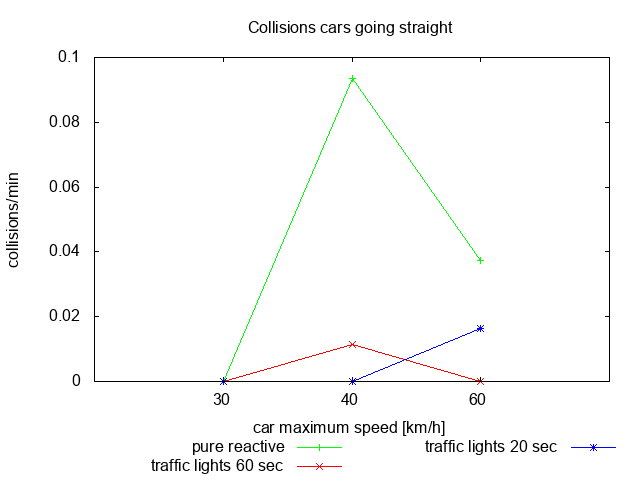
\includegraphics[scale=0.35]{img/plot_collisionsstraight}
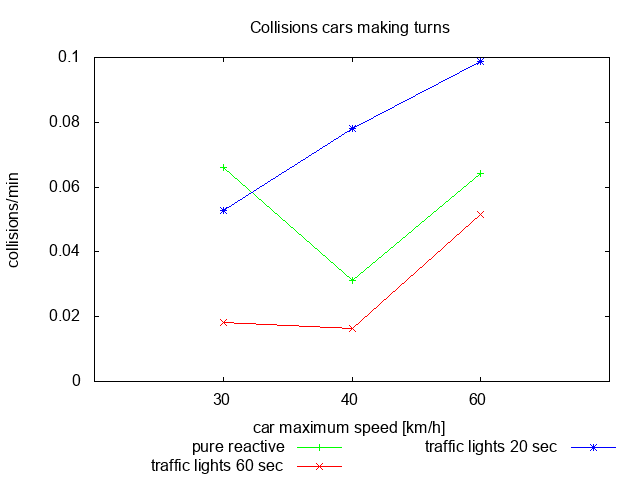
\includegraphics[scale=0.35]{img/plot_collisionsturns}
\caption{Collisions in comparison}
\label{fig:collisions}
\end{figure}




